\chapter{Анализ задачи}

\section{Общий анализ}

Система управления должна позволять контролировать множество приложений. Для её
реализации лучше всего подходит клиент-серверная архитектура. Для каждого
целевого приложения будет запускаться отдельный клиент, который будет заниматься
сбором информации об элементах управления и передавать её на сервер.

В качестве сервера будет выступать приложение, которое запускает целевые
приложения вместе с клиентами. После этого сервер принимает входяще соединение
от клиента и отображающее окно поиска элемента для текущего активного окна.

Для удобной работы окно поиска должно отображаться окно поверх работающего
приложения. И в нем должен производится нечеткий поиск.

Подобный функционал реализован в текстовых редакторах таких как VSCode, Sublime
text, Atom и называется <<палитра команд>>.

\begin{figure}
	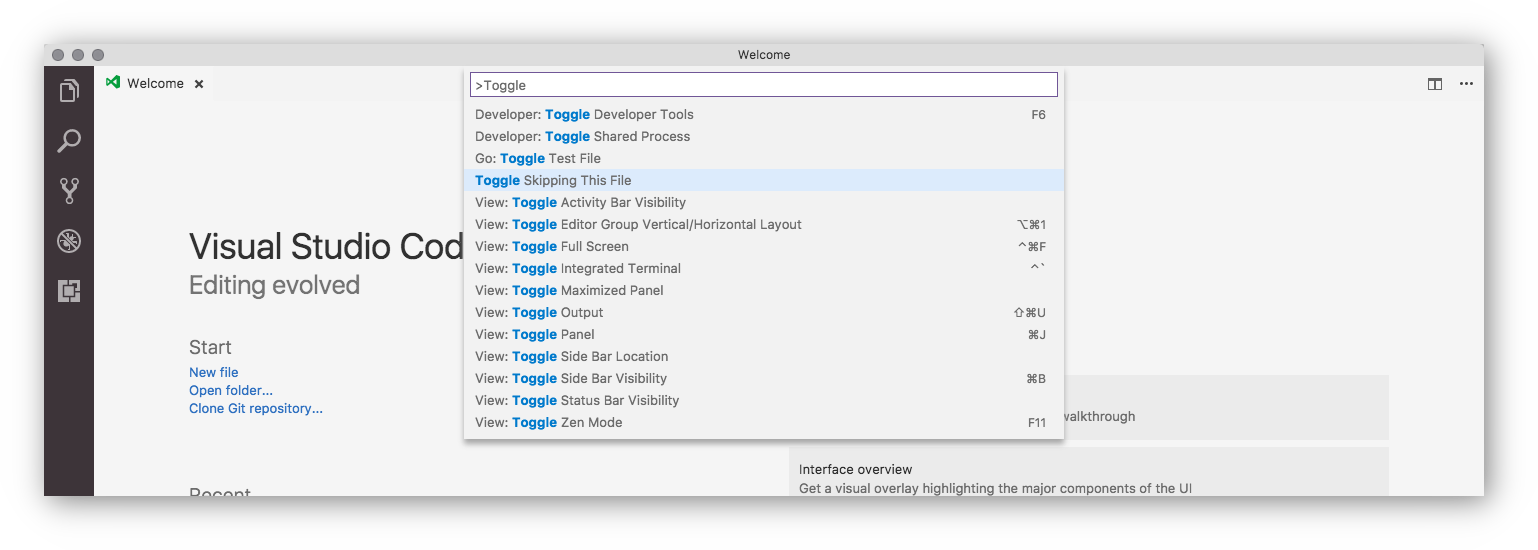
\includegraphics[width=\textwidth]{vscode}
	\caption{VSCode}
\end{figure}

\begin{figure}
	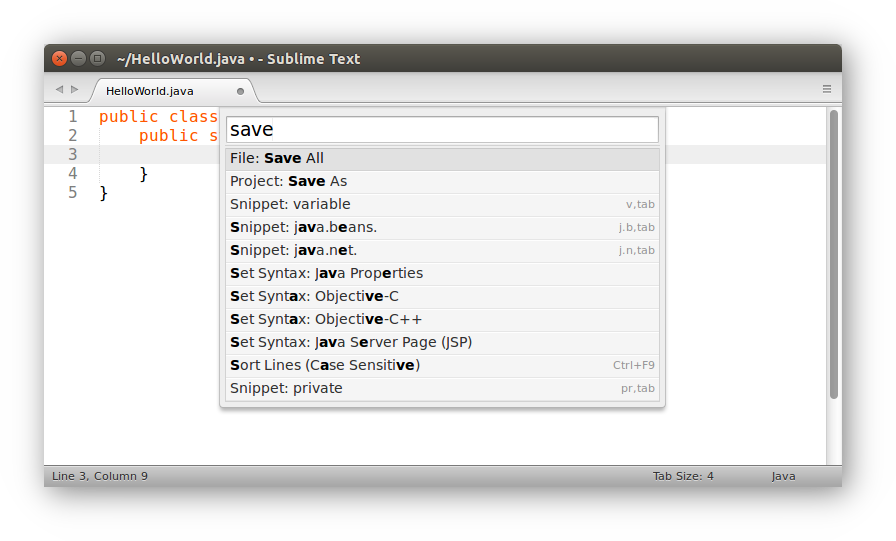
\includegraphics[width=\textwidth]{SublimeText}
	\caption{Sublime Text}
\end{figure}

В операционной системе Linux существует две основных графических библиотеки: GTK
и Qt. Библиотека GTK, начиная с третьей версии предоставляет возможность
запускать приложения с дополнительными модулями, которые могут расширять
функциональность приложения. Этим воспользовались разработчики библиотеки
Plotinus, реализовав возможность добавления палитры команд в любое приложение,
использующее GTK3.

\begin{figure}
	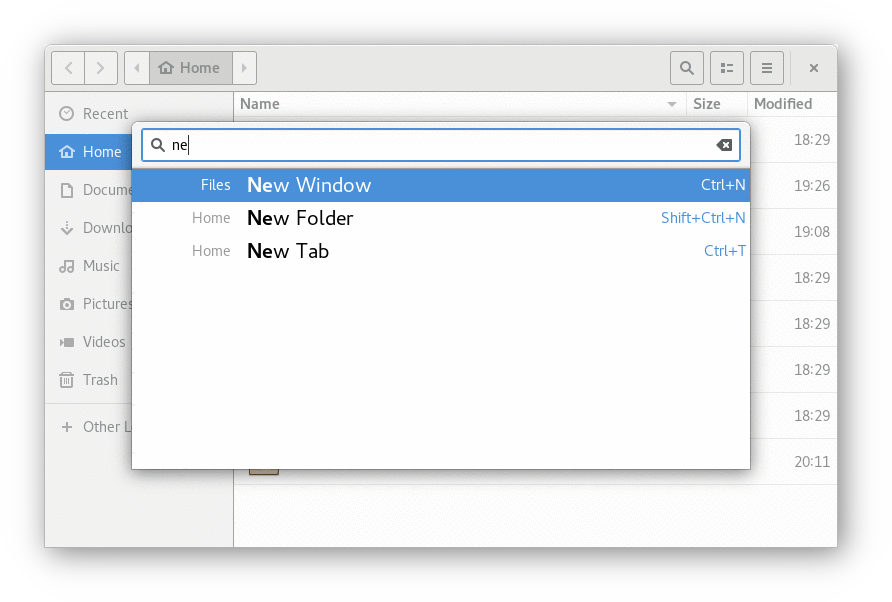
\includegraphics[width=\textwidth]{Plotinus}
	\caption{Plotinus}
\end{figure}

\subsection{Способ получения информации об элементах}

В общем случае Qt не предоставляет возможности добавить сторонний модуль в
существующую программу, поэтому для этого придется использовать средство
системы. А именно --- инъекцию динамической библиотеки.

В операционной системе Linux есть специальная переменная окружения, которая
говорит загрузчику, чтобы определенная библиотека была загружена раньше других.
Таким образом  операционная система в первую очередь загружает указанную
библиотеку, что передает вызывающей программе указатели на функции загруженной
библиотеки. Такой механизм позволяет регистрировать вызовы различных функций.

Для получения информации об элементах интерфейса можно загрузить специальную
библиотеку, которая будет регистрировать создания, изменения и удаления
элементов интерфейса. Затем собранная информация будет передавать на сервер для
последующей работы.

Пользовательский интерфейс через специальное API получает от сервера информацию
о доступных элементах в текущем приложении. После того, как пользователь
произвел выбор, вызывается специальная функция на стороне сервера, которая
приводит к отправке команды клиенту.

Клиент на своей стороне реализует возможность активации элемента интерфейса
(нажатие кнопки, выбор меню и т.п.).

\section{Постановка задачи}

Разработать набор программ, которые в комплексе будут решать следующие задачи:
\begin{itemize}
	\item запускать целевые приложения в специальном окружении;
	\item собирать информацию о существующих элементах графического приложения;
	\item сохранять информацию о всех запущенных приложениях;
	\item отображать пользователю окно для поиска и выбора элемента;
	\item активировать выбранный пользователем элемент.
\end{itemize}
